% PHẦN TRÊN HÌNH 2: 2 cột (Cột lề trống, Cột chính chứa lý thuyết)
\noindent
\begin{minipage}[t]{0.27\textwidth}
    ~ % Lề trái để trống
\end{minipage}%
\hfill
\begin{minipage}[t]{0.69\textwidth}
    \vspace{0pt}
    \setlength{\abovedisplayskip}{4pt}
    \setlength{\belowdisplayskip}{4pt}
    Một ký hiệu thay thế cho
    \[
    \lim_{x \to a} f(x) = L
    \]
    là
    \[
    f(x) \to L \quad \text{khi} \quad x \to a
    \]
    thường được đọc là “$f(x)$ tiến tới $L$ khi $x$ tiến tới $a$”.

    \vspace{0.7em}
    Hãy chú ý cụm từ “nhưng $x \neq a$” trong định nghĩa giới hạn. Điều này có nghĩa là khi tìm giới hạn của $f(x)$ khi $x$ tiến tới $a$, chúng ta không bao giờ xét $x = a$. Trên thực tế, $f(x)$ thậm chí không cần phải xác định khi $x = a$. Điều duy nhất có ý nghĩa là $f$ được xác định \emph{ở gần} $a$ như thế nào.

    \vspace{0.7em}
    Hình 2 thể hiện đồ thị của ba hàm số. Lưu ý rằng ở phần (b), $f(a)$ không xác định và ở phần (c), $f(a) \neq L$. Nhưng trong mỗi trường hợp, bất kể điều gì xảy ra tại $a$, luôn đúng là $\lim_{x \to a} f(x) = L$.
\end{minipage}

\vspace{1.2em}

% HÌNH 2: Trải dài toàn bộ chiều rộng trang
\noindent
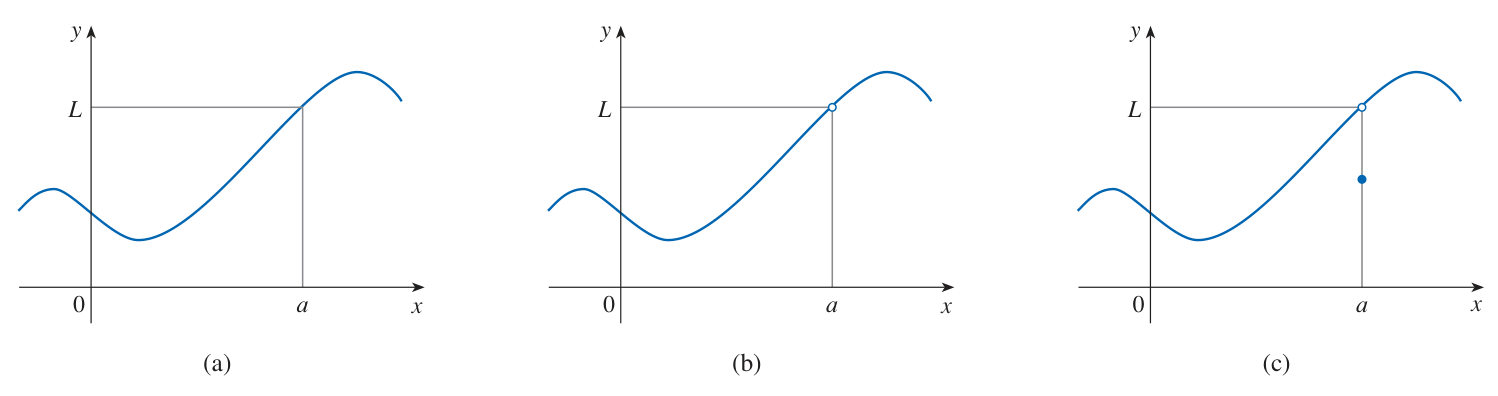
\includegraphics[width=\textwidth]{images/p0119_fig1.png}

\vspace{1.0em}

% PHẦN DƯỚI HÌNH 2: 2 cột (Cột lề chứa caption & bảng nhỏ, Cột chính chứa Ví dụ 1 & lời giải)
\noindent
\begin{minipage}[t]{0.27\textwidth}
    \vspace{0pt}
    \raggedright
    \textbf{\textsf{HÌNH 2}}\par
    \vspace{2pt}
    $\lim\limits_{x \to a} f(x) = L$ trong cả ba trường hợp

    \vspace{7.2cm}
    \begin{center}
    \renewcommand{\arraystretch}{1.25}
    \small
    \begin{tabular}{|c|c|}
    \hline
    \rowcolor{stewarttablehead}
    $t$ & $\dfrac{\sqrt{t^2 + 9} - 3}{t^2}$ \\
    \hline
    $\pm 0.001$ & $0.166667$ \\
    $\pm 0.0001$ & $0.166670$ \\
    $\pm 0.00001$ & $0.167000$ \\
    $\pm 0.000001$ & $0.000000$ \\
    \hline
    \end{tabular}
    \end{center}
\end{minipage}%
\hfill
\begin{minipage}[t]{0.69\textwidth}
    \vspace{0pt}
    \noindent\textbf{\textsf{\color{stewartcyan}VÍ DỤ 1}}\quad Ước lượng giá trị của $\lim\limits_{t \to 0} \dfrac{\sqrt{t^2 + 9} - 3}{t^2}$.

    \vspace{0.8em}
    \noindent\textbf{\textsf{\color{stewartcyan}LỜI GIẢI}}\quad Bảng dưới đây liệt kê các giá trị của hàm số với một vài giá trị của $t$ ở gần 0.

    \vspace{0.5em}
    \begin{center}
    \renewcommand{\arraystretch}{1.25}
    \begin{tabular}{|c|c|}
    \hline
    \rowcolor{stewarttablehead}
    $t$ & $\dfrac{\sqrt{t^2 + 9} - 3}{t^2}$ \\
    \hline
    $\pm 1.0$ & $0.162277\dots$ \\
    $\pm 0.5$ & $0.165525\dots$ \\
    $\pm 0.1$ & $0.166620\dots$ \\
    $\pm 0.05$ & $0.166655\dots$ \\
    $\pm 0.01$ & $0.166666\dots$ \\
    \hline
    \end{tabular}
    \end{center}

    \vspace{0.5em}
    Khi $t$ tiến tới 0, các giá trị của hàm số dường như tiến tới $0.166666\dots$ và vì vậy chúng ta đoán rằng
    \[
    \lim_{t \to 0} \frac{\sqrt{t^2 + 9} - 3}{t^2} = \frac{1}{6}
    \tag*{{\color{stewartcyan}\rule{1.1ex}{1.1ex}}}
    \]

    \vspace{0.6em}
    Trong Ví dụ 1, điều gì sẽ xảy ra nếu chúng ta chọn các giá trị của $t$ thậm chí còn nhỏ hơn nữa? Bảng ở lề trang cho thấy các kết quả từ một máy tính cầm tay; bạn có thể thấy rằng dường như có điều gì đó kỳ lạ đang diễn ra.

    \vspace{0.8em}
    Nếu bạn thử thực hiện các phép tính này trên chính máy tính của mình, bạn có thể nhận được các giá trị khác nhau, nhưng cuối cùng bạn sẽ nhận được giá trị 0 nếu bạn làm cho $t$ đủ nhỏ. Liệu điều này
\end{minipage}
